\documentclass[11pt,letterpaper]{article}
\usepackage[margin=0.85in]{geometry}
\usepackage[T1]{fontenc}
\usepackage{xurl}
\usepackage{mathptmx,amsmath,amssymb,booktabs,array,ragged2e,xcolor,microtype,hyperref,fancyhdr,longtable,pgfplots}
\pgfplotsset{compat=1.18}
\definecolor{studyblue}{RGB}{39,83,109}
\hypersetup{colorlinks=true,urlcolor=studyblue,citecolor=studyblue,linkcolor=black,pdfauthor={Jonathan Yantis},pdftitle={Beyond USB Packet Arrival: Frame-Identified Time Transfer to macOS}}
\setlength{\parindent}{1em}\setlength{\parskip}{3pt}\setlength{\headheight}{14pt}\setlength{\emergencystretch}{2em}
\widowpenalty=10000\clubpenalty=10000
\renewcommand{\floatpagefraction}{0.8}\renewcommand{\topfraction}{0.9}\renewcommand{\textfraction}{0.08}
\pagestyle{fancy}\fancyhf{}\fancyhead[L]{\small USB Frame Time Transfer to macOS}\fancyhead[R]{\small Review preprint, 15 October 2026}\fancyfoot[C]{\small\thepage}
\newcommand{\ns}{\,\mathrm{ns}}\newcommand{\us}{\,\mu\mathrm{s}}\newcommand{\ms}{\,\mathrm{ms}}\newcommand{\ppm}{\,\mathrm{ppm}}
\newcommand{\code}[1]{\texttt{#1}}\newcolumntype{L}[1]{>{\RaggedRight\arraybackslash}p{#1}}

\begin{document}
\title{\vspace{-1.4em}Beyond USB Packet Arrival:\\Frame-Identified Time Transfer to macOS}
\author{Jonathan Yantis\\\small Engineer}
\date{Research preprint, revised 15 October 2026\\\small Final USB / user-level chrony experiment; not submitted}
\maketitle
\begin{abstract}
A user-level clock can follow an embedded reference without steering the operating system clock or using USB packet arrival as a timestamp. We capture full-speed USB frame boundaries in hardware, identify their host-frame counterparts independently of clock fitting, and compose a causal counter-to-Mach map with an immutable source map and a retained UTC translation. The fine estimate feeds a private chronyd instance on macOS. In a completed 300.065 s experiment, qualified pre-ingest base-USB counter forecasts achieved 328.413 ns RMS across 9,437 observations. In the predeclared 60--300 s settled window, chrony's reported estimator RMS ranged 23--339 ns (median 129 ns,265 queries). A separate common-instant comparison of the delivered clock with its fine source estimate measured 414.351 ns RMS, with 182 valid and 54 withheld observations; its maximum absolute difference was 1.315$\mu$s. There were no USB request errors or actual daemon restarts. We explain the resolved repeated UTC-translation defect, the fit and authority contracts, and the remaining availability and calibration work. These results establish sub-microsecond settled relative RMS on one setup; shared-source agreement and an internal estimator do not independently establish absolute UTC accuracy.
\end{abstract}

\section{Introduction}
The useful timestamp is the time of an event, even when the packet describing it arrives later. This study brings an embedded BLE-derived clock to a macOS application over USB. TC-01 supplies time to the TC-04 receiver over BLE; the Mac receives only USB. A hardware-captured USB start-of-frame (SOF) event links the receiver's counter to the Mac's Mach clock. USB control transfers carry the captured evidence, rather than supplying the phase observations through their callback times.

The implementation now supplies an experimental fine UTC estimate to a private user-owned chronyd instance and reads back its virtual clock. The operating system clock is unchanged. The clock's source is the BLE-derived USB refclock, identified as BLE; chronyd reports Stratum 1 when it selects that source. Stratum is a hierarchy indicator, not a statement of calibrated accuracy. The integration discovers compatible USB timing relays on any port; the present experiment tests TC-04 on one direct full-speed XHCI connection.

Three measurements answer different questions. A pre-ingest USB forecast tests the causal bridge using only preceding observations. Chrony's reported tracking RMS describes its internal estimate. A simultaneous delivered-clock-minus-fine-estimate difference measures the application's agreement with its own source. We report all three, their populations, and the availability denominator. The main result is a usable sub-microsecond settled RMS clock estimate with stable daemon operation, while startup, occasional withheld output and absolute endpoint bias remain explicit.

Earlier work on this setup found quiet short-window monotonic phase but millisecond variation in reported UTC. Code review traced repeated noise to recomputing an integer UTC translation from coarse observations independently of the fine monotonic map. Binding that translation to one coherent source interpretation removed the repeated variation in the final capture. The original experiment remains valid historical evidence, rather than the description of the current result.
\section{Related work and comparison criteria}\label{sec:related}
\subsection{gPTP, PTP and the Mac clock endpoint}
IEEE 802.1AS specifies timing and synchronization for time-sensitive networks, using IEEE 1588 mechanisms where applicable. The IEEE working group's current published list includes 802.1AS-2025; historical evaluations below use their stated earlier editions \cite{as2025}. gPTP supplies a network timing architecture with synchronization messages, rate relationships and link-delay handling. The USB prototype in this paper does not implement its message set, peer-delay machinery, election or conformance requirements. The conceptual connection is the transport of event timestamps and the need to cross clock domains without treating software delivery delay as event phase.

A particularly relevant implementation is Clark's \emph{mac-gptp}. It exposes a Mac's AVB gPTP virtual clock through the private TimeSync framework and can feed a chrony reference-clock socket. Its documented setup uses an AVB-capable Ethernet path and a Linux boundary clock. The README reports roughly 250 ns agreement between successive Mach/gPTP mapping estimates over a few seconds and explicitly retains uncertainty in a fixed adapter-to-Mach cross-timestamp offset \cite{macgptp}. This is closely related to our host-endpoint problem, despite the different transport and API.

The project's refclock account reports 0.6 $\mu$s RMS over half an hour with tuned chrony settings and approximately 2 $\mu$s excursions during its fastest wander. It identifies oscillator wander by comparing the Mac mapping with a separate adapter-clock mapping and explains the importance of short frequency-estimation histories \cite{macrefclock}. These are author-reported system-clock-to-gPTP residuals, not our measurements and not a calibrated UTC benchmark. We did not run that project, configure AVB, or steer the system clock. Its distinct adapter clock also provides an attribution experiment that our USB run lacks: our relative rate changes cannot yet be assigned uniquely to the Mac, USB reference, TC-04 or its upstream source.

Val et al. evaluate an FPGA-based Ethernet/wireless TSN clock-domain translation with an external Calnex measurement. Their Table III reports $-4.3\ns$ mean and $18.7\ns$ standard deviation for a three-hop Ethernet setup, and $-5.5\ns$ mean and $16.6\ns$ standard deviation for one 802.11 plus two Ethernet hops \cite{val}. These are externally observed synchronization distributions in their implementation, not residuals after independently fitting short intervals. The numerical similarity of any short-window figure in our study would not establish an equivalent result.

NIST's calibration study illustrates the missing metrology more directly. Technical Note 2030 reports a 36 ns maximum offset through two transparent clocks with a 6 ns one-sigma uncertainty, and separately discusses source calibration and a power-related anomaly that increased receiver-calibration uncertainty to 100 ns \cite{nist2030}. This is evidence for the importance of reference calibration, not a performance baseline that our experiment can claim to meet.

\subsection{USB synchronization and causal delay bounds}
Lim, Rosdi and Yap use USB 3.0 Isochronous Timestamp Packets to coordinate device triggering. Their publisher abstract reports approximately 200 ns trigger delay and operation through up to three consecutive hubs \cite{lim}. The endpoint is relative triggering among SuperSpeed devices, rather than a full-speed device-to-Mach clock association. It is nevertheless clear prior evidence that USB timing can be much finer than a software transaction interval. Patent literature also describes recovering and synthesizing device clocks from periodic USB structures \cite{usbpatent}; we do not present SOF-based synchronization as a new general principle.

WALT's primary clock-synchronization notes develop causal upper and lower clock-offset bounds from messages in both directions. They report interval widths around 100 $\mu$s on one Linux USB 2 path and 800 $\mu$s on a USB 3 path \cite{walt}. Those are bound widths on named configurations, not standard deviations or physical accuracy floors. We use a related causal principle for \emph{integer identity}, while hardware boundary observations supply the fine phase evidence. Our periodic UTC request intervals deliberately remain wide rather than pretending that a request midpoint is an exact event time.

NTP is a separate network clock-discipline system. RFC 5905 discusses capabilities extending to tens of microseconds on suitable workstations and fast LANs \cite{ntp}. The Internet pool checks in our experiment do not test that regime. A noisy network observation is not evidence that the underlying NTP-disciplined clock is noisy by the same amount.


\section{Timing architecture and coordinate contracts}
Let $C$ be the receiver's free-running counter, $M_g(C)$ the source-monotonic projection for immutable map generation$g$, and $O$ its retained integer UTC translation. The source coordinate is
\begin{equation}U(C)=M_g(C)+O.\end{equation}
Let $A$ denote Mach absolute time, $K$ Mach continuous time, and $W$ local macOS wall time. These coordinates have separate meanings and failure boundaries. The USB bridge estimates $A=F(C)$ from hardware SOFs. To evaluate source time at a current host event, the client uses the inverse causal map $C=F^{-1}(A)$ and applies the exact eligible $M_g$ and $O$. A bracketed association relates $A$ to$K$; local $W$ is used to deliver the SOCK sample and interpret the daemon's clock, not to train the SOF fit.

\subsection{Hardware capture and transport}
TC-04 uses an nRF52840 TIMER3 at 16 MHz (62.5 ns ticks). A USBD SOF event triggers PPI capture into CC3, so a delayed userspace callback cannot move the original hardware timestamp. Nordic documents a synchronization stage before PPI; timer resolution does not calibrate that stage or the physical USB path\cite{nordic}. Capture records preserve the timer, frame ordinal, scope and epoch. Acceptance requires coherent frame sampling, strictly advancing sequence/counter, a consistent frame increment and capture age below 16,000 ticks (one full-speed frame).

Vendor EP0 requests retrieve precision SOF/source records at 32 Hz and periodic source information at 1 Hz. The tested interface is FF/54/01, not a standard USB time class. UTS1 kind 1 uses request 0x53; kind 2 uses 0x52. Marker OUT 0x54 and immutable fetch IN 0x55 carry a nonce-bound 64-byte marker tuple. The helper uses the public IOUSBHost APIs, including \code{referenceMicroframeWithTime:error:}; runtime Mach conversion is 125/3 ns per tick on this setup\cite{appleusb,appleframe}. The 1 ms frame cadence and 125$\mu$s microframe numbering are event spacings, not accuracy floors for timestamped edges.

\subsection{Identify the frame before fitting phase}
A smooth affine fit cannot distinguish two host/device associations separated by a whole frame. The implementation therefore constrains the integer host-microframe origin using causal zero-data OUT marker transactions and separately recorded host frame-layout checks. Request and completion brackets bound when the marker could have been observed; the marker fetch retrieves the immutable captured tuple later. On this direct full-speed XHCI topology, the intersection of these bounds identifies one integer origin. A 1$\mu$s model allowance is part of this identification procedure; it is not an independently calibrated total uncertainty bound.

The bridge requires at least eight valid layout checks and sixteen causal markers, verifies the omission of the three microframe bits in the full-frame API, and retains expiry and consistency fences. A frame-origin change, boot change, USB/capture epoch change or invalid host association invalidates the affected model. Matching this identity is distinct from estimating fine phase. Sleep/resume, hubs and alternate controllers have not been qualified by this experiment.

\subsection{Fit a clock using its past}
The shipping bridge retains at most 1,024 accepted SOF tuples, approximately 32 s at the requested rate. A causal forecast requires at least 64 prior points. For a tuple$(C_i,A_i)$, the prior window gives $F_{i-1}$; the counter-to-host innovation is evaluated before the tuple is ingested. Only then may the model be refitted. The qualified inverse-counter forecast population additionally applies the existing hardware and eligibility checks. Its signed error is expressed in nanoseconds; it is not a retrospective fitted residual.

For signed errors$e_i$, we report
\begin{equation}
 \overline e=\frac 1N\sum_i e_i,\qquad
 \mathrm{RMS}=\sqrt{\frac 1N\sum_i e_i^2},\qquad
 \sigma=\sqrt{\frac 1N\sum_i(e_i-\overline e)^2}.
\end{equation}
RMS keeps bias. A whole-run detrend, a last-window residual, a forward innovation and an inverse forecast are different populations. In particular, the final 1,024-point fitted residual is not substituted for full-capture prediction performance. No request midpoint, local-wall residual or future tuple trains the fine bridge.

\subsection{Source permission remains original}
Each usable source record carries the exact map, full root/boot/source/path scope and original permission deadline. The client evaluates whether the captured or projected counter lies in that map's interval and clips host use to the original deadline. A later map cannot retroactively authorize an unavailable event. Source restart, interpretation change, invalid UTC, malformed input, unknown classifications and original expiry retain their withdrawal fences.

The .53 correction distinguishes missing historical-SOF geometry from current source withdrawal. Under the existing publication lock, a reason 7/USM1 classification is emitted only when projecting the current counter under the same original source map succeeds. Its flags and captured UTC remain zero: it is an invalid time sample. The host withholds output and cancels pending sends while retaining private filter training only within the old grant's unchanged deadline and exact provenance. This observation cannot extend permission or install a new UTC map. True withdrawal and expiry still discard the relevant state. No GM behavior or authority deadline was changed by this RC/host correction.

\section{User-level chrony integration}
The normal CLI starts one owned private chronyd 4.9 instance with \code{-x -U -u CURRENT\_USER}, a private command socket and a SOCK refclock. The documented \code{-x} mode disables system-clock adjustment\cite{chrony}. The local manager uses a contained known configuration, waits for both sockets, and reaps only its own child. No administrator service, system timing configuration or direct Mac Bluetooth receiver is involved. Compatible relay discovery spans USB ports; identity checks and exclusive ownership prevent accidental mixed-device records.

The default fine feed composes the causal SOF/Mach bridge, the immutable source projection and the retained UTC translation at a common host instant. Integer UTC differences avoid epoch-sized floating-point subtraction. Each admitted fine observation retains a wall/Mach bracket no wider than 2$\mu$s, its original grant deadline, source generation and packet provenance. This admission limit does not become a 2$\mu$s absolute accuracy claim. A generation fence cancels pending feeds on authority transitions.

The application monitors chrony's tracking correction and rate to project its user-level clock in local wall coordinates, subject to Mach freshness and wall-step guards. The recorded SOCK configuration uses \code{poll 0 filter 4 precision 0.05 delay 0.2}, with \code{minsamples 4} and \code{maxsamples 64}. The 50 ms precision and 200 ms delay are provisional configured allowances, not measured uncertainty bounds or tracking RMS. The SOCK refclock has stratum 0; the observed selected virtual clock reports stratum 1. No forced local stratum, fabricated PPS, trust override or network fallback creates a successful selection. Tracking RMS is the daemon's historical offset statistic\cite{chrony}; the UI labels it CHRONY EST RMS and uses whole nanoseconds below 1$\mu$s.

Presentation and authority remain separate. For a display glitch strictly shorter than 500 ms, the large clock/RMS hold the last visible values with an immediate loss indicator; at 500 ms the outage presentation applies. Held pixels never feed chrony or serve clock APIs. The chrony page exposes source, frequency, freshness, filter/feed and lifecycle statistics. A smooth screen is not evidence of continuous time availability.

\section{Experiment and predeclared analysis}
The final trial ran for 300.065 s using firmware 0.15.53 (commit \path{1a16110a662ae66109b21bafa9958baf48d0465a}) and the frozen CLI 0.21 package. The operator date is 15 October 2026; capture launch was 16 October 2026 at 04:08:13 UTC. Hardware is one Apple silicon Mac, macOS 26.7 build 25G229, and one direct full-speed XHCI connection to TC-04 following TC-01. Selected source scope remained constant. RF/GNSS placement, temperature and load were not controlled treatment variables.

Before capture, the test declared full $0\le t<300$s and settled $60\le t<300$s windows. The settled boundary is not selected from the observed convergence trace. New tracking queries and fresh selected status estimates are counted separately; zero-update intervals are not selectively removed. Approximately 1 Hz status samples supply explicit valid/withheld denominators. Missing observations are not filled and their counts do not imply measured continuous outage durations.

The direct comparison computes delivered chrony UTC minus the fine estimate at the same admitted host wall/Mach instant, using integer differences. This is a shared-source relative comparison: source or endpoint error common to both clocks may cancel. It is independent of chrony's reported RMS statistic, but it is not an independent UTC reference. The trial disabled external NTP queries and made no operating-system clock changes.

Exact reviewed app-only installation preceded the run: actual new-application bytes, all 672 protected blocks and supported identical-UF2 unattended return were verified. The fixed helper budget was 9,600 samples. It completed at 299.990533 s; the following USB-session fence and daemon epoch end were planned finite cleanup, with no successor daemon. All samples in the fixed windows, including the final cleanup milliseconds, remain retained. This is not an unplanned source outage or an actual restart. Owned processes, descriptors, sockets, writers and locks were closed after the run.

\section{Results}
\subsection{Current base USB prediction}
Table\ref{tab:usb} gives the final capture's base bridge results. The complete shipping replay runs forward over the unchanged raw capture. This recovers the final three hardware tuples beyond the last live status snapshot, without retroactively training any forecast. The native end record resets the bridge during finite cleanup; its zero counters are not the capture's performance summary.

\begin{table}[htbp]\centering\small
\caption{Base USB bridge, complete final capture. Forecasts use preceding data.}\label{tab:usb}
\begin{tabular}{L{0.61\linewidth}r}\toprule Measurement & Result\\\midrule
Hardware tuples: accepted / rejected &9,558 /42\\
Qualified pre-ingest inverse forecasts &9,437\\
Inverse forecast RMS / population $\sigma$ &328.413 /314.672 ns\\
Inverse forecast mean / minimum / maximum & $-94.003/-897.863/+722.899$ns\\
Separate forward innovations: $N$ / RMS &9,494 /327.448 ns\\
Forward innovation population $\sigma$ &313.840 ns\\
Final 1,024-point fitted residual $\sigma$ (diagnostic) &103.409 ns\\
Whole-run detrended counter $\sigma$ / relative drift &4.527$\mu$s /$+5.602$ppm\\
Host frame-layout checks / failures &1,200 /0\\
Accepted / rejected causal markers &1,198 /2\\\bottomrule
\end{tabular}\end{table}

Of 9,600 raw hardware tuples,9,558 were accepted and 42 rejected. Qualified inverse forecasts numbered 9,437;24 were rejected by hardware validation and 139 were skipped or unqualified. Their RMS was 328.413 ns with bias retained. Separate forward phase innovations gave 327.448 ns RMS. These two similar values are not pooled. The whole-run 4.527$\mu$s detrended counter spread shows the slower rate wander that a local causal fit follows. The final 103.409 ns rolling fitted residual describes only its current window.

All 9,866 valid source records carried one identical UTC translation; its observed range was zero. Source-map mismatch count was zero. The removed repeated translation noise is therefore absent in the current observed scope. A constant translation can still carry an unknown initial bias.

\subsection{Chrony estimator and delivered clock}
Table\ref{tab:chrony} separates chrony's reported estimator from the application's direct comparison. All 265 new tracking queries in the settled window were below 1$\mu$s RMS. Their median was 129 ns,95th percentile 263 ns by nearest rank, and last value 98 ns. The separate fresh selected status population numbered 182 and had median 128.5 ns and 95th percentile 278 ns. Repeated observations of a filter statistic are not independent accuracy trials.

\begin{table}[htbp]\centering\small
\caption{Predeclared settled window, $60\le t<300$s.}\label{tab:chrony}
\begin{tabular}{L{0.63\linewidth}r}\toprule Statistic / population & Result\\\midrule
New tracking queries &265\\
Reported tracking RMS: minimum / median / maximum &23 /129 /339 ns\\
Reported tracking RMS: P95 / last &263 /98 ns\\
Direct chrony-minus-fine comparison: valid / withheld &182 /54 of 236\\
Direct comparison RMS / population $\sigma$ &414.351 /413.841 ns\\
Direct comparison signed bias / maximum absolute &$-20.549$ns /1.315$\mu$s\\
Source-valid / withheld status observations &235 /1 of 236\\
USB request errors / actual daemon restarts &0 /0\\\bottomrule
\end{tabular}\end{table}

The delivered-clock comparison achieved 414.351 ns RMS across 182 valid points, with 54 withheld of 236 status observations. Its maximum was 1.315$\mu$s: sub-microsecond RMS does not mean every difference was below 1$\mu$s. The full 0--300 s population had 220 valid comparisons and 76 withheld of 296, with 399.373 ns RMS. Chrony's initial tracking RMS reached 32.072201 ms; that startup transient is retained in Figure\ref{fig:tracking} and is not folded into a claim that all readings were sub-microsecond.

\begin{figure}[htbp]\centering
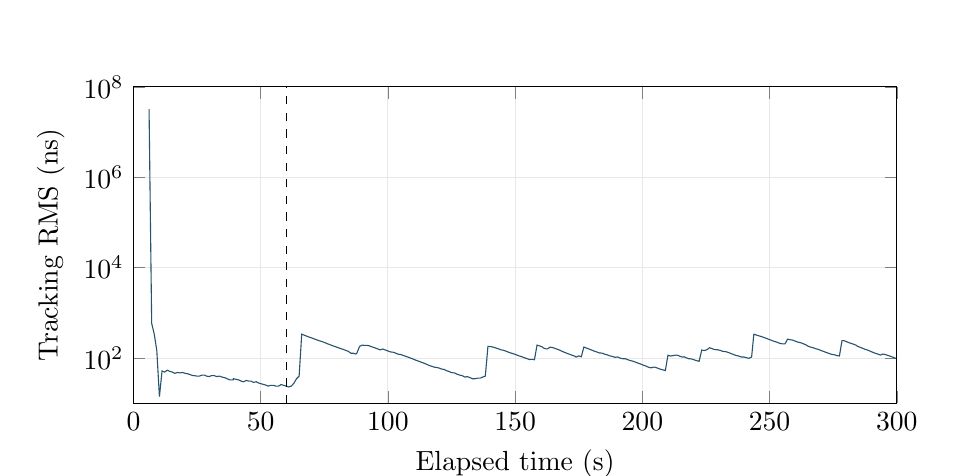
\begin{tikzpicture}\begin{semilogyaxis}[width=.93\linewidth,height=5.6cm,xmin=0,xmax=300,ymin=10,ymax=100000000,xlabel={Elapsed time (s)},ylabel={Tracking RMS (ns)},grid=major,grid style={gray!18},log basis y=10]
\addplot[studyblue,mark=none,thin] coordinates {(6.139754,32072201.000000) (7.167496,587.000000) (8.188968,336.000000) (9.182648,146.000000) (10.214984,14.000000) (11.242265,52.000000) (12.263655,49.000000) (13.263431,54.000000) (14.264421,51.000000) (15.295277,49.000000) (16.287763,46.000000) (17.294130,48.000000) (18.309659,47.000000) (19.315500,48.000000) (20.314328,46.000000) (21.341971,45.000000) (22.346786,43.000000) (23.364732,41.000000) (23.886093,41.000000) (24.889960,40.000000) (25.913493,40.000000) (26.946116,42.000000) (27.941319,42.000000) (28.686717,40.000000) (28.711360,40.000000) (29.713372,39.000000) (30.718550,41.000000) (31.738281,41.000000) (32.768867,39.000000) (33.793565,40.000000) (34.810556,38.000000) (35.809215,37.000000) (36.819613,35.000000) (37.843217,33.000000) (38.867941,33.000000) (39.209981,33.000000) (39.257311,35.000000) (40.266826,34.000000) (41.289602,33.000000) (42.285170,31.000000) (43.293627,30.000000) (44.295700,32.000000) (45.322556,31.000000) (46.191977,31.000000) (47.194401,29.000000) (48.214928,30.000000) (49.242037,28.000000) (50.239694,27.000000) (51.259841,26.000000) (52.296494,25.000000) (52.944583,24.000000) (52.961237,24.000000) (53.972223,25.000000) (54.986084,25.000000) (55.996248,24.000000) (57.010942,24.000000) (58.013962,26.000000) (59.015672,25.000000) (60.035877,24.000000) (61.042895,23.000000) (62.071059,24.000000) (63.086547,28.000000) (64.092212,35.000000) (65.115125,40.000000) (66.135907,339.000000) (67.136168,321.000000) (68.141449,305.000000) (69.157954,290.000000) (70.164482,278.000000) (71.161935,265.000000) (72.188506,251.000000) (73.214525,240.000000) (74.213766,231.000000) (75.212754,220.000000) (76.235343,208.000000) (77.238585,198.000000) (78.263175,188.000000) (79.288828,180.000000) (80.318326,171.000000) (80.391156,171.000000) (80.409715,171.000000) (81.418721,162.000000) (82.435334,156.000000) (83.439922,148.000000) (84.457425,141.000000) (85.483882,128.000000) (86.381535,128.000000) (86.414482,128.000000) (87.435671,123.000000) (87.814510,130.000000) (87.837180,130.000000) (88.858043,181.000000) (89.838464,194.000000) (89.882615,194.000000) (90.890332,191.000000) (91.912473,191.000000) (92.915641,185.000000) (93.915265,176.000000) (94.945638,168.000000) (95.967327,160.000000) (96.987381,152.000000) (97.995976,159.000000) (99.010340,151.000000) (100.009611,144.000000) (101.016103,137.000000) (102.036834,135.000000) (103.036607,129.000000) (104.061372,122.000000) (105.089907,120.000000) (106.086529,114.000000) (107.116100,109.000000) (108.135093,104.000000) (109.135703,99.000000) (110.165959,94.000000) (111.159926,89.000000) (112.182536,85.000000) (113.186146,81.000000) (114.208653,77.000000) (115.207215,73.000000) (116.210643,69.000000) (117.216662,66.000000) (118.239775,63.000000) (119.242468,62.000000) (120.234554,60.000000) (121.236678,57.000000) (122.239182,56.000000) (122.810830,53.000000) (122.836756,53.000000) (123.860720,51.000000) (124.861873,48.000000) (125.863423,47.000000) (126.185842,47.000000) (127.187409,44.000000) (128.229257,42.000000) (129.209183,41.000000) (130.210929,38.000000) (131.213144,39.000000) (132.236763,37.000000) (133.260840,35.000000) (134.186299,35.000000) (134.236311,35.000000) (135.240941,36.000000) (136.234850,36.000000) (137.261272,38.000000) (138.285747,40.000000) (139.315601,182.000000) (140.334829,180.000000) (141.338324,175.000000) (142.365086,168.000000) (143.365911,161.000000) (144.382626,153.000000) (145.414745,149.000000) (146.435393,142.000000) (147.438114,135.000000) (148.460493,129.000000) (149.485099,124.000000) (150.510521,118.000000) (151.514602,112.000000) (152.538031,108.000000) (153.535522,102.000000) (154.562048,98.000000) (155.588062,93.000000) (156.588019,94.000000) (157.588370,92.000000) (158.611114,194.000000) (159.634717,186.000000) (160.660603,177.000000) (161.064476,168.000000) (161.086742,168.000000) (162.088038,160.000000) (162.686303,160.000000) (162.711452,160.000000) (163.742007,175.000000) (164.763325,171.000000) (165.762038,163.000000) (166.763212,156.000000) (167.784919,148.000000) (168.437612,141.000000) (169.460159,134.000000) (170.462595,127.000000) (171.483835,121.000000) (172.511385,115.000000) (173.512106,110.000000) (173.937339,105.000000) (173.959902,105.000000) (174.986497,112.000000) (176.007790,107.000000) (177.010755,176.000000) (178.015056,167.000000) (179.018201,159.000000) (180.036832,151.000000) (181.060559,143.000000) (182.086182,137.000000) (183.112853,130.000000) (184.139833,129.000000) (185.160748,122.000000) (186.183292,118.000000) (187.207511,112.000000) (188.234749,109.000000) (189.257906,104.000000) (190.284157,106.000000) (191.284981,100.000000) (192.287145,97.000000) (193.310429,97.000000) (194.336584,92.000000) (195.360849,88.000000) (196.383795,85.000000) (197.389732,81.000000) (198.410255,77.000000) (199.312879,74.000000) (199.336902,74.000000) (200.338909,70.000000) (201.363129,67.000000) (202.362904,63.000000) (203.392179,61.000000) (204.407412,63.000000) (204.935060,63.000000) (204.959927,63.000000) (205.985728,60.000000) (207.011349,57.000000) (208.037039,55.000000) (209.034904,53.000000) (210.058550,116.000000) (211.064583,111.000000) (212.086075,114.000000) (213.086940,116.000000) (213.685575,116.000000) (213.737937,116.000000) (214.737603,110.000000) (215.761465,105.000000) (216.385573,107.000000) (216.409194,107.000000) (217.186810,102.000000) (217.211359,102.000000) (218.236520,97.000000) (219.257114,96.000000) (220.258069,92.000000) (221.285739,88.000000) (222.309673,85.000000) (223.337690,151.000000) (224.362759,147.000000) (225.386529,153.000000) (226.410809,170.000000) (227.413920,162.000000) (228.435591,154.000000) (229.462036,153.000000) (230.492130,149.000000) (231.436926,142.000000) (231.464556,142.000000) (232.485599,139.000000) (232.813284,139.000000) (232.835210,139.000000) (233.836528,133.000000) (234.834279,126.000000) (235.862448,120.000000) (236.862594,114.000000) (237.860173,111.000000) (238.885282,106.000000) (239.892227,106.000000) (240.912531,102.000000) (241.914893,99.000000) (242.942141,106.000000) (243.812313,339.000000) (243.837111,339.000000) (244.837108,323.000000) (245.862012,310.000000) (246.861737,299.000000) (247.888115,284.000000) (248.918369,271.000000) (249.937773,257.000000) (250.966192,244.000000) (251.990124,233.000000) (253.006251,224.000000) (254.016676,212.000000) (255.042997,207.000000) (256.061550,206.000000) (257.061327,263.000000) (258.061801,255.000000) (259.087572,250.000000) (260.086833,237.000000) (261.088693,226.000000) (262.111076,220.000000) (263.134702,209.000000) (264.134834,199.000000) (265.161637,183.000000) (266.197295,175.000000) (267.218700,169.000000) (268.210583,161.000000) (269.235213,155.000000) (270.261919,147.000000) (271.291173,140.000000) (272.311573,133.000000) (273.338831,127.000000) (274.360778,121.000000) (275.389145,119.000000) (276.411835,114.000000) (277.437494,111.000000) (278.461003,244.000000) (279.107545,244.000000) (279.133290,244.000000) (280.137775,232.000000) (281.138886,220.000000) (282.159470,210.000000) (283.185564,201.000000) (284.209602,191.000000) (284.458462,183.000000) (284.507568,183.000000) (285.534728,174.000000) (286.561157,165.000000) (287.582145,156.000000) (288.588015,150.000000) (289.582251,142.000000) (290.438891,135.000000) (290.457554,135.000000) (291.490670,128.000000) (292.507593,123.000000) (293.535162,117.000000) (294.557538,123.000000) (295.611712,119.000000) (296.584802,114.000000) (297.615661,109.000000) (298.636990,104.000000) (299.644616,98.000000)};
\addplot[black,dashed] coordinates {(60,10)(60,100000000)};
\end{semilogyaxis}\end{tikzpicture}
\caption{All positive new tracking-RMS queries in the full window. Logarithmic ordinate retains the 32.072 ms startup transient. Dashed line is the predeclared 60 s settled boundary; no transient exclusion changes that boundary.}\label{fig:tracking}
\end{figure}

\begin{figure}[htbp]\centering
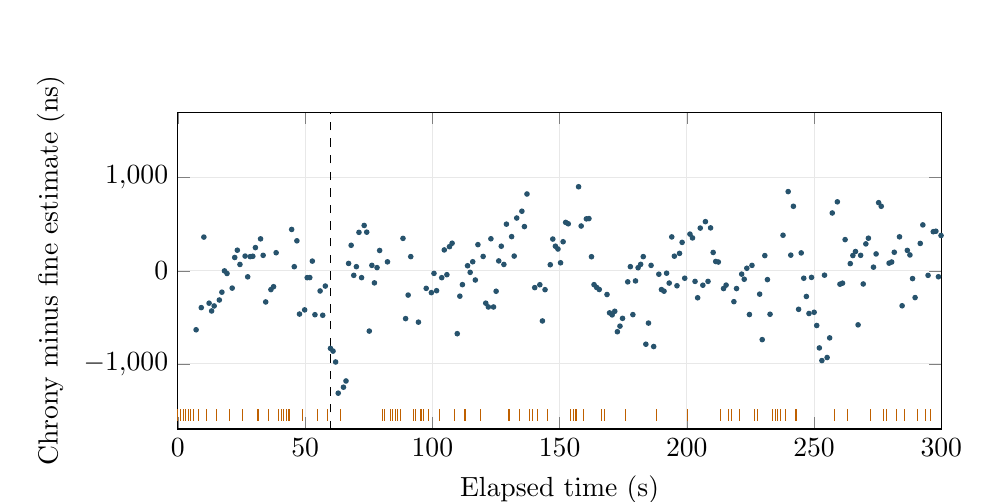
\begin{tikzpicture}\begin{axis}[width=.93\linewidth,height=5.6cm,xmin=0,xmax=300,ymin=-1700,ymax=1700,xlabel={Elapsed time (s)},ylabel={Chrony minus fine estimate (ns)},grid=major,grid style={gray!18}]
\addplot[studyblue,only marks,mark=*,mark size=.8pt] coordinates {(7.153956,-634) (9.178550,-396) (10.204221,362) (12.253556,-348) (13.254042,-432) (14.254079,-378) (16.278520,-314) (17.286287,-230) (18.303515,-1) (19.304052,-29) (21.333468,-186) (22.333648,143) (23.354017,221) (24.378465,68) (26.410002,158) (27.428463,-65) (28.432409,152) (29.433043,156) (30.453909,249) (32.478525,343) (33.503923,166) (34.503970,-335) (36.554101,-202) (37.584229,-171) (38.604016,194) (44.709695,444) (45.731119,44) (46.761713,322) (47.783218,-465) (49.809567,-420) (50.811431,-74) (51.829456,-73) (52.832158,104) (53.854125,-472) (55.882303,-217) (56.904085,-478) (57.933638,-164) (59.956448,-834) (60.959430,-863) (61.980894,-980) (63.004180,-1315) (65.060297,-1251) (66.061471,-1184) (67.078543,79) (68.083868,274) (69.109107,-49) (70.136283,44) (71.154087,413) (72.178577,-74) (73.203111,487) (74.203985,415) (75.209241,-648) (76.231461,58) (77.231848,-130) (78.258317,34) (79.284337,218) (82.358061,96) (88.453938,348) (89.482506,-514) (90.482658,-261) (91.503971,152) (94.528477,-552) (97.578596,-189) (99.610172,-235) (100.636948,-28) (101.653923,-214) (103.678527,-74) (104.681864,224) (105.704258,-42) (106.728537,259) (107.754007,296) (109.778554,-676) (110.803516,-273) (111.806597,-149) (113.830489,54) (114.853993,-17) (115.854017,97) (116.880906,-99) (117.904029,281) (119.953951,154) (120.981094,-348) (122.003994,-389) (123.004017,344) (124.031395,-389) (125.054055,-220) (126.078497,106) (127.079879,264) (128.103490,68) (129.104999,501) (131.153980,367) (132.153995,158) (133.156194,567) (135.178490,640) (136.178489,475) (137.178684,825) (140.228505,-181) (142.230125,-150) (143.253919,-539) (144.280457,-203) (146.330487,65) (147.330510,341) (148.353920,264) (149.353984,234) (150.378525,86) (151.378597,312) (152.380971,520) (153.404120,505) (157.454015,903) (158.478496,481) (160.529996,558) (161.530979,561) (162.531284,151) (163.531481,-149) (164.554003,-179) (165.581121,-201) (168.631154,-255) (169.631173,-452) (170.654000,-474) (171.681231,-435) (172.705928,-655) (173.730348,-595) (174.730516,-511) (176.778494,-119) (177.804003,44) (178.804035,-471) (179.831657,-109) (180.854010,33) (181.854019,69) (182.878508,152) (183.904067,-789) (184.931100,-562) (185.953991,58) (186.978531,-814) (189.004031,-37) (190.028505,-202) (191.031188,-219) (192.054066,-26) (193.078511,-132) (194.078579,364) (195.104073,157) (196.130653,-161) (197.131690,187) (198.154033,305) (199.178453,-80) (201.227771,394) (202.231107,353) (203.231193,-114) (204.253961,-290) (205.280074,459) (206.303987,-155) (207.304025,528) (208.328518,-114) (209.328518,461) (210.353985,197) (211.356302,100) (212.381090,94) (214.431077,-191) (215.431815,-154) (218.503981,-332) (219.530545,-191) (221.554026,-36) (222.554022,-91) (223.578527,27) (224.604001,-470) (225.604015,58) (228.628570,-251) (229.630936,-740) (230.654017,163) (231.678586,-95) (232.703479,-467) (237.804011,382) (239.831136,851) (240.855651,168) (241.881479,693) (243.930613,-414) (244.953985,192) (245.954017,-80) (246.978606,-276) (248.003527,-459) (249.004132,-71) (250.030146,-446) (251.054058,-588) (252.078486,-829) (253.078557,-965) (254.104070,-47) (255.130657,-932) (256.131145,-721) (257.154007,621) (259.154035,741) (260.178536,-144) (261.179708,-133) (262.204006,335) (264.231039,77) (265.255705,164) (266.280929,207) (267.304076,-581) (268.306283,166) (269.328529,-142) (270.353922,289) (271.354004,350) (273.354775,39) (274.378320,181) (275.378551,732) (276.404040,693) (279.478453,82) (280.503936,94) (281.531028,199) (283.578523,365) (284.604010,-376) (286.653998,219) (287.678499,170) (288.704018,-84) (289.704051,-288) (291.730303,294) (292.754034,493) (294.803992,-49) (296.854009,420) (297.878473,425) (298.881257,-64) (299.904023,379)};
\addplot[orange!75!black,only marks,mark=|,mark size=2pt] coordinates {(0.003009,-1550) (1.008759,-1550) (2.030786,-1550) (3.053967,-1550) (4.081399,-1550) (5.104084,-1550) (6.132940,-1550) (8.178571,-1550) (11.233519,-1550) (15.278510,-1550) (20.304877,-1550) (25.384138,-1550) (31.458447,-1550) (35.532512,-1550) (39.634991,-1550) (40.653940,-1550) (41.656370,-1550) (42.678488,-1550) (43.678786,-1550) (48.809221,-1550) (54.879645,-1550) (58.933675,-1550) (64.032582,-1550) (80.311456,-1550) (81.336597,-1550) (83.382828,-1550) (84.403989,-1550) (85.407732,-1550) (86.411612,-1550) (87.432454,-1550) (92.508368,-1550) (93.510854,-1550) (95.533245,-1550) (96.559544,-1550) (98.606284,-1550) (102.654026,-1550) (108.778531,-1550) (112.830445,-1550) (118.930700,-1550) (130.130558,-1550) (134.178482,-1550) (138.203940,-1550) (139.205956,-1550) (141.229600,-1550) (145.304048,-1550) (154.406550,-1550) (155.430275,-1550) (156.431601,-1550) (159.504002,-1550) (166.604005,-1550) (167.629527,-1550) (175.754112,-1550) (188.003477,-1550) (200.203986,-1550) (213.404023,-1550) (216.454046,-1550) (217.480355,-1550) (220.553940,-1550) (226.604251,-1550) (227.605829,-1550) (233.704219,-1550) (234.731335,-1550) (235.754037,-1550) (236.778506,-1550) (238.830102,-1550) (242.904207,-1550) (258.154057,-1550) (263.230527,-1550) (272.354031,-1550) (277.430035,-1550) (278.453973,-1550) (282.555956,-1550) (285.628558,-1550) (290.705280,-1550) (293.778511,-1550) (295.830442,-1550)};
\addplot[black,dashed] coordinates {(60,-1700)(60,1700)};
\end{axis}\end{tikzpicture}
\caption{Every valid full-window shared-source comparison, with withheld status observations shown as orange ticks at$-1550$ns (their vertical position is a plotting key, not an error value). No line interpolates missing observations. Settled RMS is 414.351 ns, and the observed maximum absolute difference is 1.315$\mu$s.}\label{fig:delivery}
\end{figure}

\subsection{Transport, provenance and remaining availability}
The capture recorded 2,102 successful fine feeds, zero feed errors/quarantines, zero USB request/transport errors, zero helper restarts and zero source rotations. Independent reconstruction found 9,866 genuine source grants, exactly matching native acceptance. All 2,102 feed provenance checks and 291 fine-observation deadline/bracket/integer checks passed without violations. These checks verify the recorded contract, not timing truth between recorded events.

The settled source was valid in 235/236 status observations, yet direct delivery was available in 182/236. Of the 54 withheld comparisons,45 had an unidentified delivery gate (in-flight feeder work is possible), seven had stale reference, one lacked a current anchor and one lacked source permission. The log does not expose the feeder-busy predicate; the 45 cannot be conclusively attributed to that path. Counts are point-sampled availability, not a continuous coverage guarantee. Improving this interface is more urgent than advertising a smaller internal RMS number.

\section{Discovery, corrections and separate historical evidence}
\subsection{Repeated UTC translation noise: found and resolved}
The earlier 600 s build recomputed \code{utc\_offset\_ns = utc - ns} in radio publication from fresh coarse/raw UTC observations while the precise source-monotonic map evolved independently. Its reported UTC phase had 1.465 ms detrended variation despite quiet short-window monotonic phase. Review localized and corrected this concrete publication behavior in the accepted .51 source change (commit\path{5b7087d}).

The time owner now binds one integer translation using a coherent uptime/counter observation within 100$\mu$s, retains that interpretation across ordinary map/publication revisions, and applies it consistently to precision publication, preferred JOIN and serving display. Contradictory or invalid associations and source restart fence before replacement. The existing 2 s contradiction threshold is a rejection policy, not an accuracy bound. The final 9,866 valid records show one retained translation, resolving the repeated translation variation in this run. Initial PPS/RMC second association and fixed bias still require independent commissioning; this change does not create a verified UTC anchor or repair genuine GNSS reception loss.

\subsection{USB continuity and map classification}
The .52 USB fix addresses pinned EP0 busy/ZLP retirement and superseded completion generations. The original physical trigger of the earlier startup hang was not established. The .53/CLI.21 change adds the bounded missing-SOF classification described above, preserving invalid-sample refusal and original expiry. Focused C/native checks and a real private-daemon synthetic lifecycle test cover brief retention, unchanged old deadline, true withdrawal, malformed input and required recycling.

The previous separate 300 s .52/CLI.20 trial had zero USB errors but 46 actual chrony restarts,47 precision-only no-map responses and 103 valid/133 withheld settled comparisons. Its settled direct comparison RMS was 414.137 ns. The final run has zero restarts and 182 valid/54 withheld, while direct RMS stays 414.351 ns. The observed improvement is daemon continuity and sampled deliverability, not a reduction in already sub-microsecond direct agreement. No natural reason 7, retention, refusal or original-expiry event occurred in the final run. Therefore the new classification's physical branch coverage and its causal responsibility for the restart improvement are not proved by this comparison. RF/GNSS and temperature were uncontrolled and may have differed between sequential trials; populations are not pooled.

\subsection{Earlier 600 s base-USB experiment}
The original 600.013 s phase-only experiment is retained as a separate method/history population. It had 19,093 accepted hardware tuples and 18,332 valid source observations. All 20 disjoint 30 s windows had detrended phase$\sigma$ below 0.288$\mu$s (median 0.155$\mu$s). Fitting each preceding 30 s block and predicting the next without refit gave 1.053$\mu$s RMS,3.285$\mu$s absolute P99 and 3.662$\mu$s maximum across 17,439 predictions. A single full-run fit left 3.956$\mu$s source$\sigma$ and$+4.635$ppm drift. Window choice was exploratory after capture. Those retrospective/local-block results are not the current causal 328 ns forecast or the current chrony statistic.

Ten historical read-only NTP checks had reported uncertainty$\pm 52.884$--$\pm 96.552$ms, too broad to calibrate this USB endpoint. No matched NTP or gPTP comparison was performed in the final trial. The earlier millisecond UTC variation is discovery evidence, not an unresolved description of the corrected current stream. Earlier raw failures, source gaps and rejected observations remain preserved in their original archives.

\section{Limits and room for improvement}
\subsection{What the final results establish}
The final run establishes a causal base-USB RMS near 328 ns and a settled delivered user-clock agreement RMS near 414 ns, on one composite TC-01/TC-04/Mac path. It demonstrates a practical userspace chrony integration without operating-system clock control. It does not measure independent UTC error. Shared-source/common-mode error can cancel, chrony's tracking RMS is internal, and unique frame identity,62.5 ns timer ticks and a narrow admission bracket are not a full uncertainty budget. Apple/controller/PHY/cable-to-Mach offset, the source's initial UTC bias and qualified PPS/RMC second association remain unknown.

There is one finite direct-XHCI trial, with no controlled alternate-Mac, hub, suspend/reconnect, thermal or CPU/I/O stress cohort. GNSS/RF conditions were not independently recorded as metrology truth. The experiment covers neither leap-second behavior nor adversarial source integrity. Exclusive USB ownership and identity checks avoid accidental mixing; they are not cryptographic authentication of an attached malicious device. Absolute UTC traceability, continuous precision availability, long-run durability and superiority over NTP/gPTP are not claimed.

\subsection{A concrete next sequence}
First, instrument every delivered-clock refusal with an explicit gate reason and admission generation. Investigate whether a stable atomic snapshot can permit ordinary same-authority updates without an unnecessary busy refusal; preserve all reset, wall-step, source-transition and expiry fences. The 45 unidentified settled refusals are a diagnosis target, not proof that a specific gate is faulty. This aims to close the 235-source-valid versus 182-deliverable gap without extending authority.

Second, evaluate bridge-window adaptation against frozen causal criteria, with controlled load and temperature and fresh validation runs. Report bias, RMS, tails and availability together. The difference between the whole-run 4.527$\mu$s counter variation and 328 ns causal forecast supports following local rate, but does not by itself select a universally optimal window. Do not substitute the final 103 ns fitted residual for an end-to-end result.

Third, independently commission the PPS-to-UTC association and calibrate the physical endpoint/Mach bias. A second timed host event or external reference is needed to expose errors shared by the fine feed and chrony. Finally, compare USB, NTP and gPTP at a common independently timed endpoint with matched horizons and availability. The comparisons in related work motivate those experiments; unlike-for-like published values do not rank transports.

\section{Conclusion}
The corrected stream supports a working macOS user-level clock. In the declared settled window, reported chrony estimator RMS remained 23--339 ns, and direct delivered-clock agreement with its fine source was 414.351 ns RMS. The base USB bridge separately achieved 328.413 ns qualified pre-ingest forecast RMS. There were zero USB request errors and zero actual daemon restarts. Binding the UTC translation removed the repeated coarse-to-fine publication noise observed earlier, while causal fitting followed slower relative rate variation. The next engineering priority is delivery availability; independent endpoint and UTC calibration are the next metrology priorities.

\section*{Data, code and reproducibility}
This is a local research preprint, not a submitted or accepted paper. The companion \path{paper/usb-macos-evidence-20261015.json} records exact metrics, separate capture hashes and software versions. The final raw JSONL SHA-256 is \path{c401eb777976634f7717aeb9637530d111dd72525142661cbaf474aba13022d3}. Its sealed run identifier is \path{MACOS_SOF_MAP_FIVE_MINUTE_20261015_01}; the baseline is \path{MACOS_FIVE_MINUTE_20261015_01}. Historical identifiers \path{TC04_DIRECT_USB_600S_20261015_01} and \path{TC04_SHORT_WINDOW_STABILITY_20261015_01} remain separate.

The standalone LaTeX source embeds every plot coordinate and the bibliography. Derived CSVs contain elapsed time and relative measurements without physical identities or epoch-sized UTC labels. The derivation checks all rows in the fixed windows and retains withheld markers. Raw captures, protected readbacks, private sockets and hardware identifiers remain outside website assets. New CLI images replay the actual last eligible fresh status at 299.904023 s through the native renderer; only the preview's duration is corrected from 600 to 300 s. They are labeled replays, not physical display captures. Build, literature, claim-review and figure manifests accompany the review package. No public raw-data release or off-host archival guarantee is asserted.

\section*{Author contributions and assistance disclosure}
Jonathan Yantis supplied the hardware, original protocol/firmware, experimental direction and research decisions. OpenAI Codex assisted implementation, tooling, literature research, evidence review, analysis, figure/table generation, writing and LaTeX preparation. The same Sol 6.1 Extra High implementation engineer reviewed this revision's claims against code and final capture evidence. No AI system is listed as a human coauthor. The human author retains responsibility for the evidence, claims, references, privacy and any venue requirements. No affiliation, acceptance, DOI or arXiv identifier is claimed.

\begin{thebibliography}{99}\small
\bibitem{prior} J. Yantis with disclosed OpenAI Codex assistance, \emph{Passive Precision Time over BLE: V14 Boundary Clocks, Causal Timestamping, and Prospective One-Relay Validation}, local review preprint, 12 October 2026. Repository \path{paper/ptob-v14-preprint.tex}. Prior radio evidence is not pooled into this USB result.
\bibitem{as2025} IEEE 802.1 Working Group, \emph{IEEE Std 802.1AS-2025: Timing and Synchronization for Time-Sensitive Applications}, published-standard listing and maintenance project scope. \url{https://1.ieee802.org/tsn/}; \url{https://1.ieee802.org/maintenance/802-1as-2025-revision-timing-and-synchronization-for-time-sensitive-applications/}. Accessed 15 October 2026. Public project material inspected; no claim of a clause-by-clause conformance review.
\bibitem{macgptp} J. Clark, \emph{mac-gptp: Use gPTP on macOS for timing}, README and implementation documentation, commit \path{e133922d72282e1a41835a19e575663d292a21c5}, 4 September 2026. \url{https://github.com/jclark/mac-gptp/tree/e133922d72282e1a41835a19e575663d292a21c5}. Primary project report, accessed 15 October 2026; not independently reproduced here.
\bibitem{macrefclock} J. Clark, \emph{gptp-refclock}, technical notes at the same pinned revision. \url{https://github.com/jclark/mac-gptp/blob/e133922d72282e1a41835a19e575663d292a21c5/docs/gptp-refclock.md}. The reported 0.6 $\mu$s RMS is a system-clock residual against the project's gPTP reference, not calibrated absolute UTC error.
\bibitem{val} I. Val, \'O. Seijo, R. Torrego and A. Astarloa, ``IEEE 802.1AS Clock Synchronization Performance Evaluation of an Integrated Wired-Wireless TSN Architecture,'' \emph{IEEE Transactions on Industrial Informatics}, 2022, doi:10.1109/TII.2021.3106568. Author manuscript arXiv:2109.09409, 2021, Table III. \url{https://arxiv.org/abs/2109.09409}.
\bibitem{nist2030} M. A. Weiss, Y. Li-Baboud, D. Anand, K. G. Brady, P. A. Boynton, C. T. Nguyen, M. J. Burns and A. M. Gopstein, \emph{A Calibration of Timing Accuracy in the NIST Cyber-Physical Systems Testbed}, NIST Technical Note 2030, December 2018, doi:10.6028/NIST.TN.2030. \url{https://www.nist.gov/publications/calibration-timing-accuracy-nist-cyber-physical-systems-testbed-0}. The Technical Note summary, rather than the differing conference abstract, supplies the selected maximum/uncertainty wording.
\bibitem{lim} C. H. Lim, B. A. bin Rosdi and C. F. Yap, ``Synchronization of multiple USB 3.0 devices using Isochronous Timestamp Packet,'' \emph{Computer Standards \& Interfaces}, 2017, doi:10.1016/j.csi.2016.06.006. \url{https://www.sciencedirect.com/science/article/pii/S0920548916300423}. Publisher abstract/highlights inspected; full experimental article not available in this review.
\bibitem{usbpatent} P. G. Foster, \emph{USB based synchronization and timing system}, US8943351B2, 2015. \url{https://patents.google.com/patent/US8943351B2/en}. Primary disclosure of USB periodic-signal clock synchronization; a patent disclosure is not an independently reproduced benchmark.
\bibitem{walt} Google WALT contributors, ``Clock Synchronization,'' primary implementation notes preserved in Android Open Source Project. \url{https://android.googlesource.com/platform/external/walt/+/HEAD/android/WALT/app/src/main/jni/README.md}. Accessed 15 October 2026; named-machine interval widths retained as reported.
\bibitem{ntp} D. Mills, J. Martin, J. Burbank and W. Kasch, ``Network Time Protocol Version 4: Protocol and Algorithms Specification,'' RFC 5905, June 2010. \url{https://www.rfc-editor.org/rfc/rfc5905.html}.
\bibitem{nordic} Nordic Semiconductor, \emph{nRF52840 Product Specification}, v1.2, USBD isochronous transactions / SOF event and TIMER capture descriptions. \url{https://docs-be.nordicsemi.com/bundle/nRF52840_PS_v1.2/raw/resource/enus/nRF52840_PS_v1.2.pdf}. Accessed 15 October 2026; source documents 16 MHz synchronization before PPI, not a calibrated installed-device timing bias.
\bibitem{appleusb} Apple Inc., ``referenceMicroframeWithTime:error:,'' IOUSBHostObject documentation and local macOS SDK declaration. \url{https://developer.apple.com/documentation/iousbhost/iousbhostobject/referencemicroframewithtime:error:}. Accessed 15 October 2026. The public API is distinguished from DriverKit interfaces and private TimeSync.
\bibitem{appleframe} Apple Inc., ``frameNumberWithTime:,'' IOUSBHostObject documentation and local SDK declaration, accessed 15 October 2026. \url{https://developer.apple.com/documentation/iousbhost/iousbhostobject/framenumberwithtime:}. The inspected SDK explicitly describes omission of the microframe component.
\bibitem{evidence} J. Yantis with OpenAI Codex assistance, \emph{TC-04 USB and macOS chrony evidence}, sealed local experiments, 15 October 2026 operator date. Companion \path{paper/usb-macos-evidence-20261015.json} records the separate historical600s, baseline300s and final300s populations and their hashes. Raw captures are private.
\bibitem{chrony} Chrony contributors, \emph{chronyd(8)}, \emph{chronyc(1)} and \emph{chrony.conf(5)}, version 4.9 documentation. \url{https://chrony-project.org/doc/4.9/chronyd.html}; \url{https://chrony-project.org/doc/4.9/chronyc.html}; \url{https://chrony-project.org/doc/4.9/chrony.conf.html}. Accessed16 October2026 UTC. Local pinned implementation and configuration are retained with the experiment.
\end{thebibliography}
\end{document}
